\documentclass[10pt,letterpaper]{article}
\usepackage{geometry}
\geometry{margin=1in}
\usepackage{graphicx}

\setlength{\parindent}{0pt}
\setlength{\parskip}{0.5em}

\usepackage{enumitem}
\setlist{nolistsep}

\usepackage{titlesec}
\usepackage{titlesec}
\titlespacing*{\section}{0pt}{0\baselineskip}{0\baselineskip}
\titlespacing*{\subsection}{0pt}{0\baselineskip}{0\baselineskip}
\titlespacing*{\subsubsection}{0pt}{0\baselineskip}{0\baselineskip}

%reduce list spacing
\usepackage{enumitem}
\setlist{nosep}

\usepackage[hidelinks]{hyperref}

\title{Lab 3 - Parallelizing $k$-means, Stat 215A, Fall 2026\vspace{-2em}}

\date{October 2026}

\begin{document}
\maketitle

\section{Introduction}\label{introduction}

Choosing the number of clusters $k$ is a central difficulty in using $k$-means, because the algorithm returns a partition for every value of $k$ whether or not the data support it. Ben-Hur, Elisseeff and Guyon \cite{benhur2002} propose using stability as a guide. If $k$ matches real structure in the data, clustering two different random subsamples should produce similar partitions of the points the subsamples share. If it does not, the partitions should change from one subsample to the next. Stability is summarized by the distribution of a similarity score between the two clusterings, and values of $k$ whose scores concentrate near 1 are considered stable.

This procedure is applied to a binary-coded linguistic survey data set with 45,152 respondents and 468 binary columns. For each $k$ from 2 to 10, I repeat the procedure $B=100$ times, using subsamples that each contain a fraction $m=0.8$ of the respondents, so that a pair of subsamples shares about 29,000 respondents. I measure agreement with the Jaccard coefficient: the number of pairs of respondents that both clusterings place in the same cluster, divided by the number of pairs that at least one of them places together.

The main computational challenge is this similarity. With $q\approx 29{,}000$ shared respondents, the direct implementation builds a $q\times q$ matrix and takes $O(q^2)$ time, and it must be evaluated 900 times (9 values of $k$, 100 repetitions each).

\section{Similarity implementation}

\textbf{Choice of similarity.} I use the Jaccard coefficient. Ben-Hur et al.\ \cite{benhur2002} note that the matching coefficient also counts pairs of points that are apart in both clusterings, and that this term is usually dominant, so the coefficient often varies over a smaller range than the Jaccard coefficient. The Jaccard coefficient ignores those pairs, and it is close to the correlation measure that the paper uses in its own figures. It can also be computed from pair counts alone, which is what makes the fast algorithm below possible.

\textbf{Algorithm.} Let two clusterings of the same $q$ points have $k_1$ and $k_2$ clusters. Let $C^{(r)}$ be the $q\times q$ matrix with $C^{(r)}_{ij}=1$ if $i\neq j$ and points $i$ and $j$ share a cluster in clustering $r$, and $0$ otherwise. Then
\[
J=\frac{\langle C^{(1)},C^{(2)}\rangle}{\langle C^{(1)},C^{(1)}\rangle+\langle C^{(2)},C^{(2)}\rangle-\langle C^{(1)},C^{(2)}\rangle},
\qquad \langle C^{(1)},C^{(2)}\rangle=\sum_{i,j}C^{(1)}_{ij}C^{(2)}_{ij},
\]
which counts ordered pairs of points. The obvious implementation builds both matrices, which takes $O(q^2)$ time and memory; for $q\approx 29{,}000$ each matrix has about $8\times10^{8}$ entries.

The matrices are not needed. Let $n_{ab}$ be the number of points with label $a$ in the first clustering and label $b$ in the second, so $n$ is a $k_1\times k_2$ table. One pass over the $q$ labels fills it. If $r_a=\sum_b n_{ab}$ and $c_b=\sum_a n_{ab}$ are its row and column sums, then
\[
\langle C^{(1)},C^{(2)}\rangle=\sum_{a,b}n_{ab}(n_{ab}-1),\quad
\langle C^{(1)},C^{(1)}\rangle=\sum_a r_a(r_a-1),\quad
\langle C^{(2)},C^{(2)}\rangle=\sum_b c_b(c_b-1),
\]
because a group of $n$ points contains $n(n-1)$ ordered pairs. The running time is $O(q+k_1k_2)$ and the memory is $O(k_1k_2)$, so the $q\times q$ matrix is never stored. With $k\le 10$ the table has at most 100 cells, so the $O(q)$ pass dominates and the cost is essentially linear in $q$.

\textbf{Python implementation.} The final function (a single pass over the labels in a Numba-compiled loop) fills the table and the three sums with integer arithmetic, so there are no Python-level loops over points and no $q\times q$ arrays. Labels are first checked to be non-negative integers and relabeled to $0,\dots,k-1$ only if they are not, so the table is always at most $k_1\times k_2$. The first call compiles the function, so timings below are taken after a warm-up call. To show where the speed comes from, I kept four versions that return the same value: (i) a pure Python double loop over all pairs; (ii) NumPy, comparing blocks of 500 rows against all points, which is still $O(q^2)$ but uses only $O(500\,q)$ memory; (iii) the table algorithm with NumPy's \texttt{bincount}; and (iv) the table algorithm in Numba. The four versions agree on a test pair of clusterings to within $10^{-12}$.

\textbf{Timing.} For each fraction $m$ from $0.2$ to $0.8$, I drew two subsamples of the data, clustered each with $k$-means using $k=10$, and kept the $q$ points common to both (so $q$ grows with $m$; $q=1{,}788$ at $m=0.2$ and $q=28{,}965$ at $m=0.8$). All four versions were then timed on the same pair of label vectors, on my laptop. Each time is the best of three runs, where each run averages many calls; calls longer than a second were timed once. The pure Python version was run only up to $m=0.5$ (about 11,300 shared points), where a single call already took 13.5 seconds, to keep the notebook's running time reasonable.

\begin{figure}[ht]
\centering
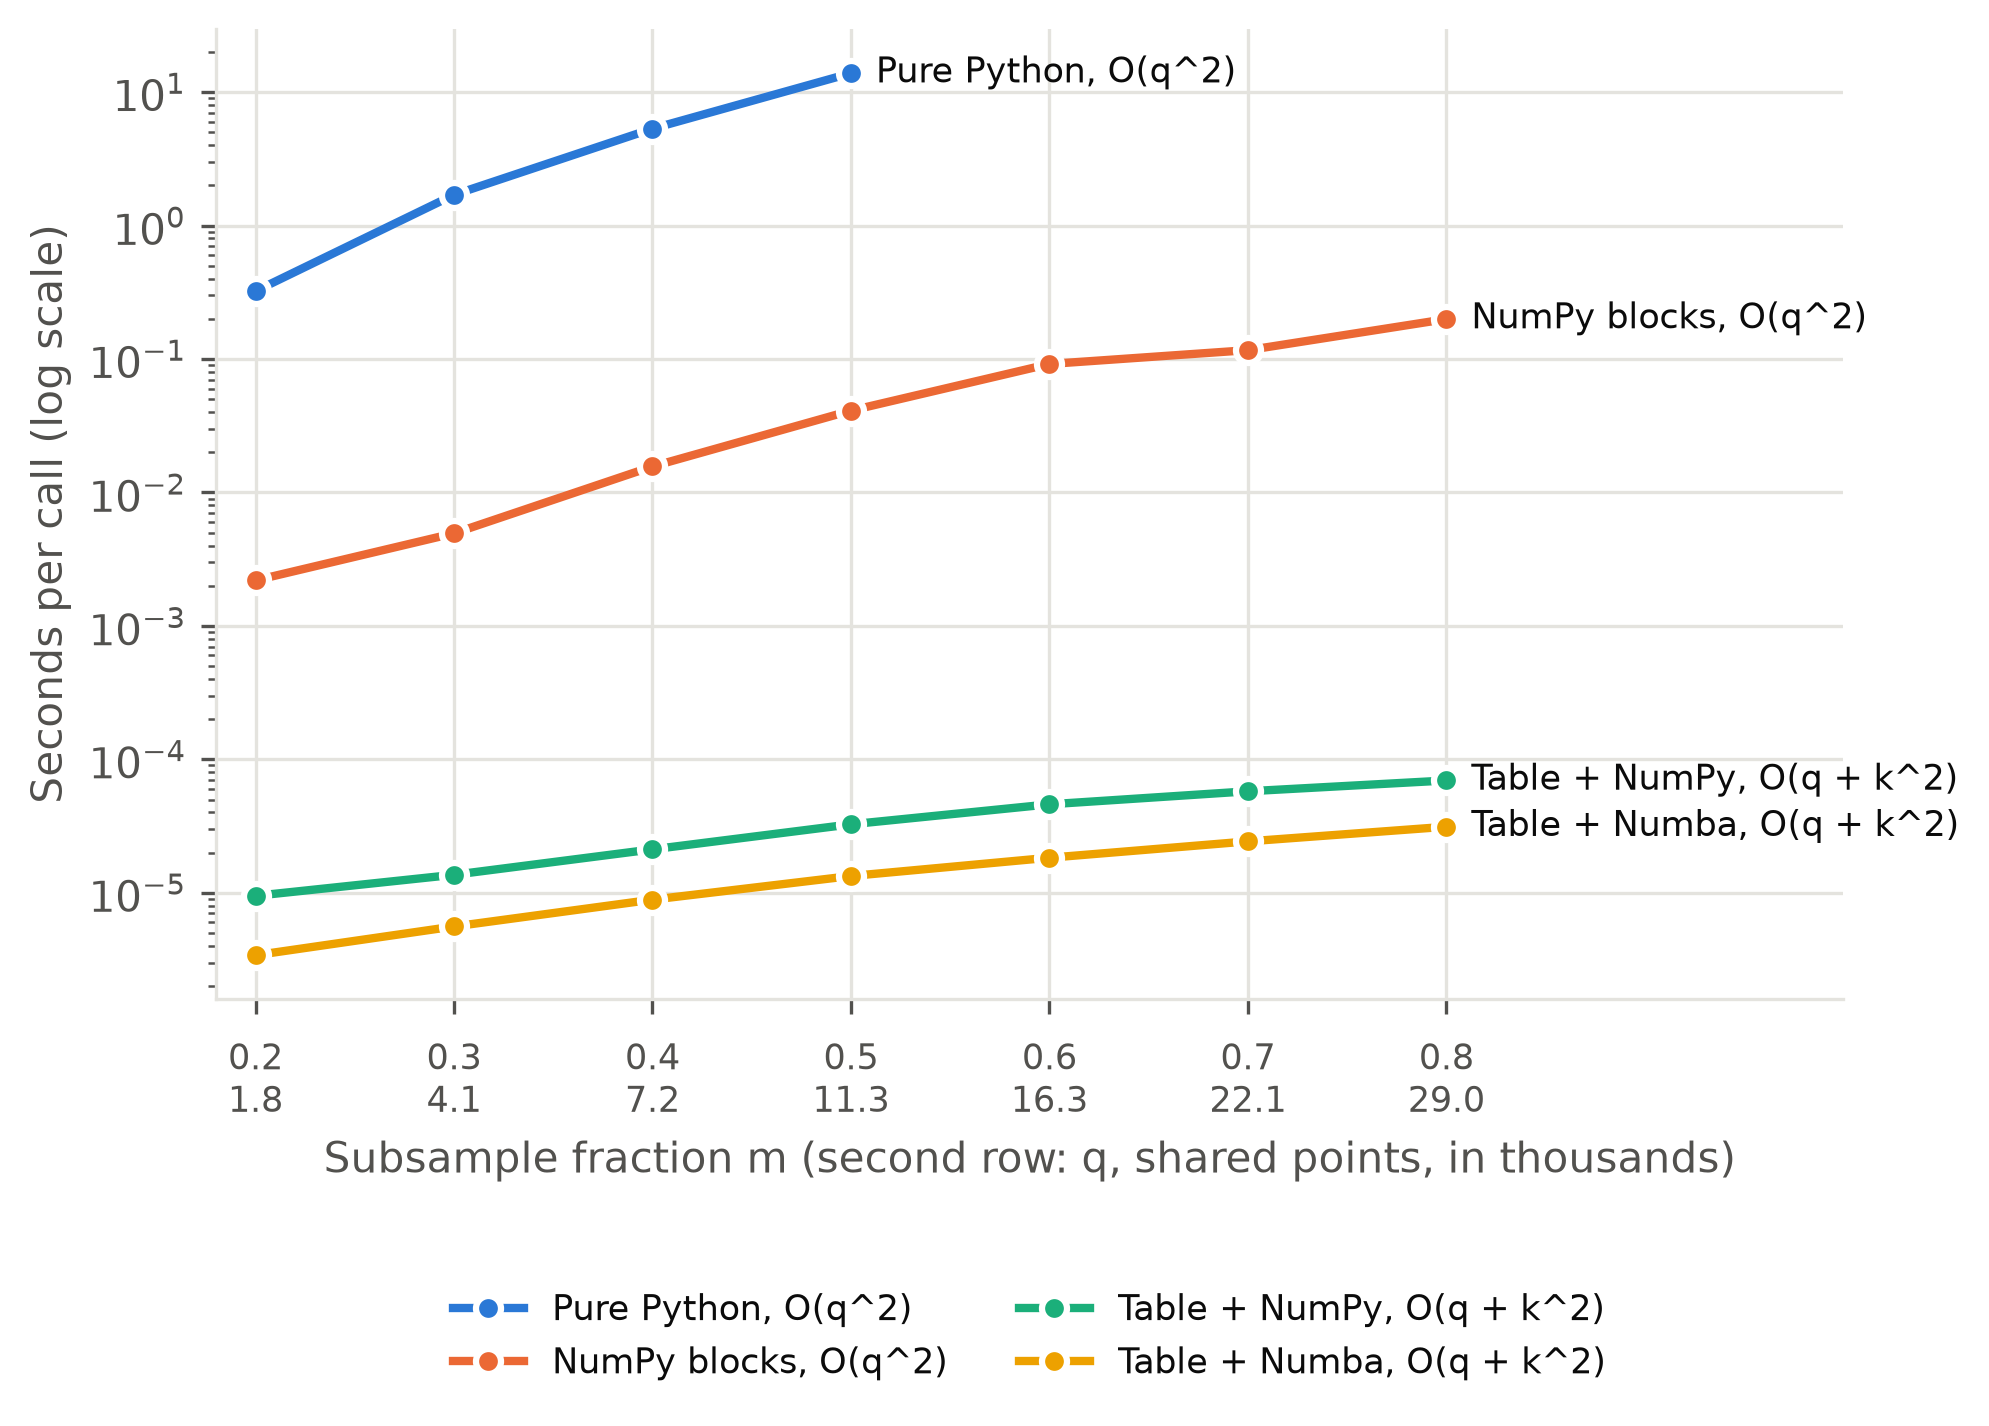
\includegraphics[width=0.8\textwidth]{figures/similarity_timing.png}
\caption{Time per similarity call against the subsample fraction $m$ (log scale). The second row of the horizontal axis gives $q$, the number of points shared by the two subsamples, in thousands. The pure Python version was not run beyond $m=0.5$.}
\end{figure}

\begin{table}[ht]
\centering
\begin{tabular}{lrrr}
\hline
 & $q=1{,}788$ & $q=11{,}279$ & $q=28{,}965$ \\
 & ($m=0.2$) & ($m=0.5$) & ($m=0.8$) \\
\hline
Pure Python, $O(q^2)$ & 0.333 s & 13.5 s & not run \\
NumPy blocks, $O(q^2)$ & 2.36 ms & 40.1 ms & 194 ms \\
Table + NumPy, $O(q+k^2)$ & 9.35 $\mu$s & 29.1 $\mu$s & 64.6 $\mu$s \\
Table + Numba, $O(q+k^2)$ & 3.44 $\mu$s & 13.1 $\mu$s & 30.5 $\mu$s \\
\hline
\end{tabular}
\caption{Time per similarity call at three values of $m$.}
\end{table}

The two $O(q^2)$ versions grow steeply: from $m=0.2$ to $m=0.4$, where $q$ roughly quadruples, the pure Python time rises about 16-fold. The two table versions rise only from a few microseconds to a few tens of microseconds while $q$ grows 16-fold, so the change of algorithm accounts for most of the speedup. At $m=0.5$, the Numba version is about a million times faster than pure Python, and at $m=0.8$ it is more than 6,000 times faster than the blocked NumPy version. Compiling with Numba gives a further factor of about 2 to 3 over the same algorithm in NumPy. At about 30 $\mu$s per call at $m=0.8$, the 900 similarity evaluations in Algorithm 1 take well under a second in total, which is negligible next to the $k$-means fits.

\section{Algorithm 1 implementation}

\textbf{Implementation.} Algorithm 1 is a separate Python script. For each $k$ from 2 to 10 and each of $B=100$ repetitions, it draws two subsamples of 36,122 respondents (a fraction $m=0.8$ of the data, drawn without replacement), clusters each with scikit-learn's \texttt{KMeans}, and computes the Jaccard similarity of the two label vectors on the respondents that appear in both subsamples, using the fast function from the previous section. The result is a $100\times 9$ matrix $S$ of similarities, saved as a CSV file. Each combination of $k$ and repetition has its own random seed, so the output does not depend on how the work is divided among cores.

\textbf{$k$-means parameters.} Apart from $k$, I used $k$-means++ initialization with a single start (\texttt{n\_init=1}) and left the maximum number of iterations (300) and the convergence tolerance ($10^{-4}$) at their scikit-learn defaults. With a single start, the difference between two clusterings includes the effect of a poor or unlucky initialization, which is part of what instability means in practice; extra restarts would reduce that noise but would multiply the running time by about the number of restarts. I chose $m=0.8$, the largest fraction the lab allows, because the full run still took only a few minutes.

\textbf{Parallelization.} The 900 combinations of $k$ and repetition are independent of one another, so they can run on separate cores. I used \texttt{joblib} with one worker process per core and limited each worker to one thread, so the workers do not compete with each other. I compared two choices. In the inner-loop version, the values of $k$ are processed one at a time and the 100 repetitions for each $k$ are spread over the workers. In the outer-loop version, each value of $k$ is one task, so there are only 9 tasks. I used the inner loop because it gives 100 tasks of similar size for each $k$. With the outer loop, at most 9 cores can be busy at once, the tasks are unequal in size (clustering into more groups generally takes longer), and the run ends only when the slowest $k$ finishes. The measured times in Table~\ref{tab:runtime} agree with this explanation, although I did not profile the workers. Both versions produce identical matrices $S$.

\textbf{Runtime and cores.} I ran the job on one node of the Savio cluster, using 24 cores (and 24 workers). Because the tasks are independent, using more cores shortens the run, and keeping everything on a single node means the workers do not need to communicate between machines. The inner-loop run took 225.5 seconds (about 3.8 minutes) and the outer-loop run took 511.7 seconds (about 8.5 minutes).

\begin{table}[ht]
\centering
\begin{tabular}{lrr}
\hline
Loop parallelized & Cores & Elapsed time \\
\hline
Inner (repetitions) & 24 & 225.5 s \\
Outer (values of $k$) & 24 & 511.7 s \\
\hline
\end{tabular}
\caption{Running time of Algorithm 1 on one Savio node for $m=0.8$, $B=100$ and $k=2,\dots,10$. Both runs give identical matrices $S$.}
\label{tab:runtime}
\end{table}

\section{Result}
\begin{figure}[ht]
\centering
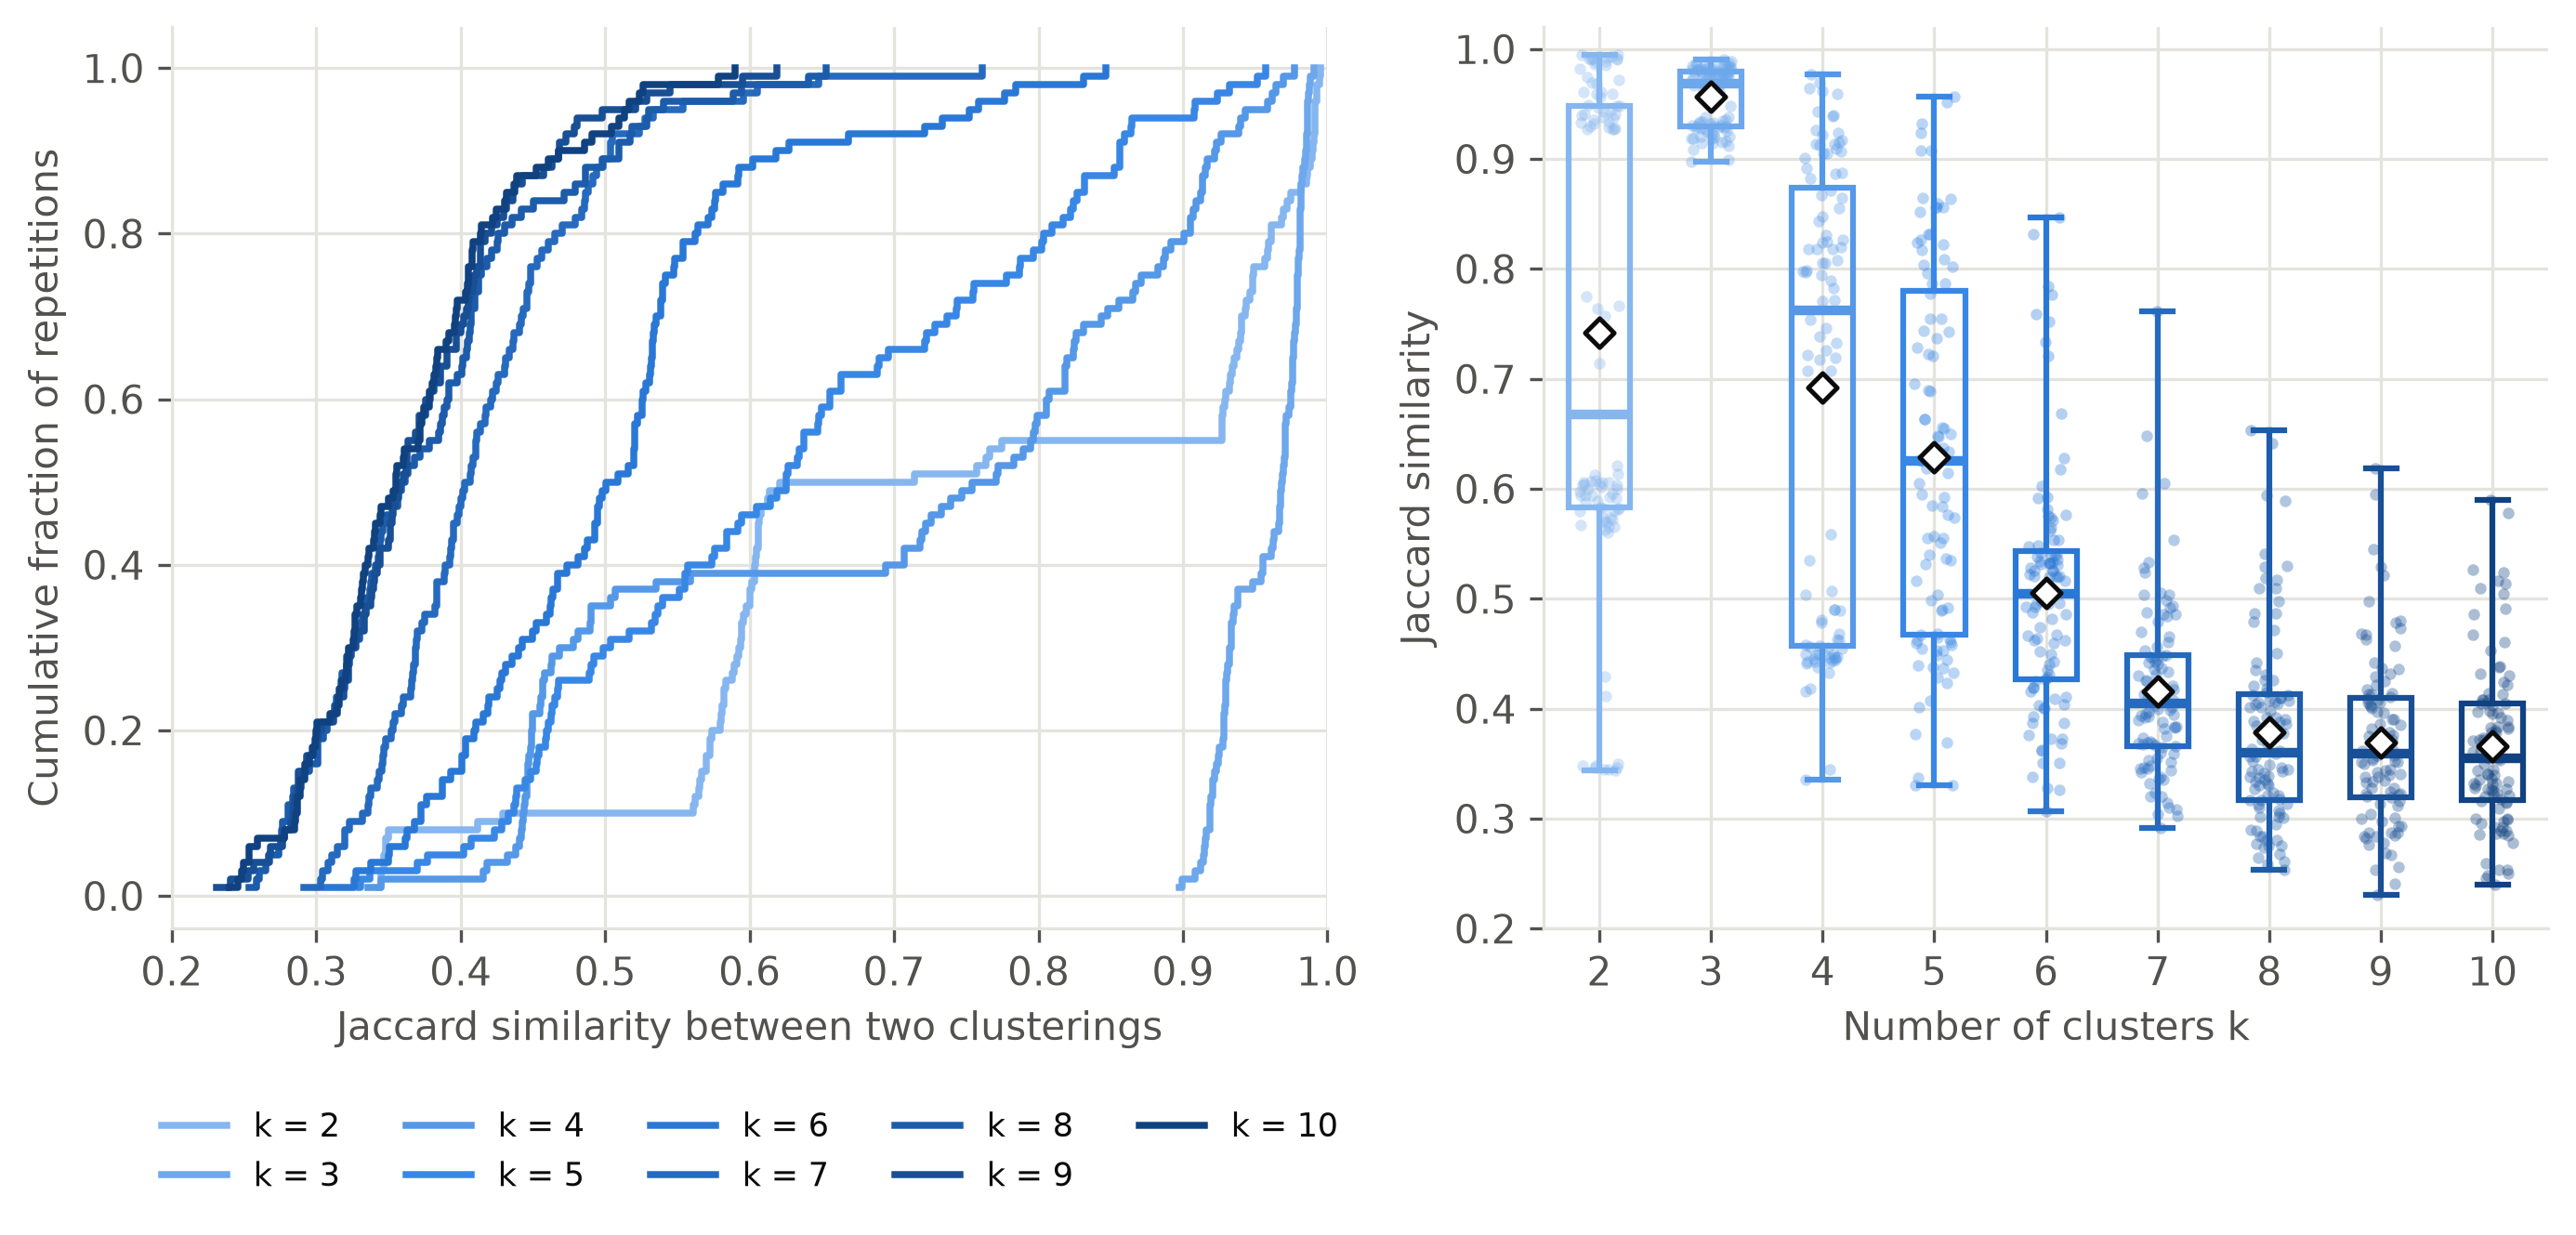
\includegraphics[width=\textwidth]{figures/stability_by_k.png}
\caption{Stability of $k$-means for $k=2,\dots,10$ ($B=100$ repetitions each, $m=0.8$). Left: empirical cumulative distribution of the Jaccard similarity between two clusterings, one curve per $k$. Right: the same 100 values for each $k$; boxes show the quartiles and median, whiskers show the minimum and maximum, the diamond is the mean and the dots are individual repetitions.}
\label{fig:stability}
\end{figure}

\begin{table}[ht]
\centering
\begin{tabular}{rccccc}
\hline
$k$ & Mean & Std.\ dev. & Min & Median & Max \\
\hline
2 & 0.742 & 0.215 & 0.344 & 0.667 & 0.995 \\
3 & 0.957 & 0.027 & 0.898 & 0.969 & 0.991 \\
4 & 0.692 & 0.202 & 0.336 & 0.762 & 0.977 \\
5 & 0.629 & 0.166 & 0.330 & 0.625 & 0.957 \\
6 & 0.505 & 0.110 & 0.307 & 0.505 & 0.846 \\
7 & 0.416 & 0.077 & 0.291 & 0.404 & 0.761 \\
8 & 0.379 & 0.086 & 0.253 & 0.360 & 0.653 \\
9 & 0.369 & 0.074 & 0.231 & 0.359 & 0.619 \\
10 & 0.366 & 0.074 & 0.240 & 0.355 & 0.590 \\
\hline
\end{tabular}
\caption{Summary of the 100 Jaccard similarities for each $k$.}
\label{tab:stability}
\end{table}

\textbf{Stability by $k$.} Figure~\ref{fig:stability} and Table~\ref{tab:stability} summarize the 100 similarity scores for each $k$. For $k=3$ the scores are concentrated near 1: all 100 are at least 0.898, 98 are at least 0.9, and the standard deviation is 0.027. At $k=2$ the scores fall into two groups: 45 of the 100 are at least 0.9, while 50 are below 0.7 and only 5 lie in between, so two subsamples sometimes agree almost perfectly and sometimes do not. At $k=4$ and $k=5$ the scores are spread widely (standard deviations 0.20 and 0.17). From $k=6$ on, no repetition reaches 0.9. The mean similarity falls from 0.957 at $k=3$ to 0.692 at $k=4$, the largest drop between consecutive values of $k$, and settles near 0.37 for $k=8$ to $10$.

\textbf{Trusting the method.} Stability measures how reproducible a partition is under subsampling. That is necessary but not sufficient for the partition to be meaningful: $k$-means can reproducibly split data along a dominant direction without the split corresponding to a real group. Several features of this analysis limit how much weight a single stability curve should carry. Two subsamples with $m=0.8$ share about 64\% of the respondents (28,965 of 45,152), so their clusterings are similar partly because they are fitted to much of the same data; a smaller $m$ would be a harder test, and I did not try one. I used a single $k$-means start, so the bimodal scores at $k=2$ and $k=4$ could reflect different local optima as well as different structure in the data. Ben-Hur et al.\ \cite{benhur2002} note that a bimodal distribution of similarities can arise when there is no single preferred partition, but I did not check with more restarts which explanation applies here. Pair counts are dominated by large clusters, so the Jaccard coefficient is less sensitive to what happens to small ones. Finally, $k$-means with Euclidean distance on 468 binary columns weights every column equally, so the result depends on that modeling choice.

\textbf{Other approaches.} Other ways to choose $k$ could be used alongside stability. The gap statistic and the silhouette width compare how compact the clusters are with a reference or with the other clusters. A mixture model for binary data lets $k$ be chosen with BIC and suits 0/1 columns better than Euclidean $k$-means. Resampling-based methods such as consensus clustering give a related but different view of stability. Agreement between several of these would be stronger evidence for a choice of $k$ than any one criterion.


\textbf{Choice of $k$.} I would choose $k=3$. Its similarity scores are both high and tightly concentrated: the mean Jaccard similarity is 0.957 with a standard deviation of 0.027, the lowest of the 100 repetitions is 0.898, and 98 of the 100 are at least 0.9. For $k=2$ the mean is 0.742 with a standard deviation of 0.215, and about half of the repetitions (45 of 100) reach 0.9 while the rest are much lower, so two subsamples often produce quite different partitions. For $k=4$ the mean falls to 0.692, the standard deviation is about 0.20 (seven times that of $k=3$), and only 21 of 100 repetitions reach 0.9. The drop from $k=3$ to $k=4$ is the sharp transition from a concentrated distribution near 1 to a wide one that Ben-Hur et al.\ \cite{benhur2002} describe as the signature of a good $k$. Beyond $k=4$ stability keeps declining, and from $k=6$ onward no repetition reaches 0.9, as stated earlier.

This shows that $k=3$ is the value for which $k$-means returns the most reproducible partition at $m=0.8$. It does not show that the respondents fall into three true groups, and I did not examine what the three clusters mean. The paper presents stability as a guide to choosing $k$, not as proof of structure.

\section{Academic Honesty}

\subsection{Statement}
Dear Bin,
I affirm that the work in this report is my own, and that all sources I used, including any discussions with
classmates, are properly cited. Academic research honesty is necessary as it is the foundation of trust in
science and the integrity of the field at large. Not only do we as researchers have an obligation to be honest
to ourselves, our labs, and the greater scientific community when it comes to research, but also to the public,
as many of us are funded by tax dollars and want our findings to be helpful to humanity.
\subsection{LLM Usage}

\subsubsection*{Coding}
Claude was mostly used for debugging and help with commenting code. 
\subsubsection*{Writing}
Claude was also used to help format in latex notation. 
\subsection{Collaborators}
Kea and I briefly chatted about our results and general lab 3 goals, but did not share code or report text at all. 
\section{Bibliography}
{\renewcommand{\section}[2]{}%
\begin{thebibliography}{9}
\bibitem{benhur2002} A.~Ben-Hur, A.~Elisseeff, and I.~Guyon. A stability based method for discovering structure in clustered data. \emph{Pacific Symposium on Biocomputing}, 7:6--17, 2002.
\end{thebibliography}
}

\end{document}